\documentclass[11pt]{article}
\usepackage[spanish]{babel}
\usepackage{natbib}
\usepackage{url}
\usepackage[utf8x]{inputenc}
\usepackage{amsmath}
\usepackage{amssymb}
\usepackage{graphicx}
\graphicspath{{images/}}
\usepackage{parskip}
\usepackage{fancyhdr}
\usepackage{vmargin}
\usepackage{natbib}
\usepackage{apalike}
\usepackage{longtable}
\usepackage{listings}
\usepackage{color}
\usepackage{pdfpages}
\usepackage{arydshln}
\usepackage{hyperref}
\hypersetup{
    colorlinks=true,
    linkcolor=black,
    filecolor=magenta,      
    urlcolor=cyan,
}

\definecolor{dkgreen}{rgb}{0,0.6,0}
\definecolor{gray}{rgb}{0.5,0.5,0.5}
\definecolor{mauve}{rgb}{0.58,0,0.82}

\lstset{frame=tb,
  language=Java,
  aboveskip=3mm,
  belowskip=3mm,
  showstringspaces=false,
  columns=flexible,
  basicstyle={\tiny\ttfamily},
  numbers=left,
  numberstyle=\tiny\color{gray},
  keywordstyle=\color{blue},
  commentstyle=\color{dkgreen},
  stringstyle=\color{mauve},
  breaklines=true,
  breakatwhitespace=true,
  tabsize=3
}

\setmarginsrb{3 cm}{2.5 cm}{3 cm}{2.5 cm}{1 cm}{1.5 cm}{1 cm}{1.5 cm}

\title{Programas}						% Title
\author{J. Eduardo Sánchez Posadas}					%Author
\date{\today}											% Date

\makeatletter
\let\thetitle\@title
\let\theauthor\@author
\let\thedate\@date
\makeatother

\pagestyle{fancy}
\fancyhf{}
\rhead{Estructuras de Datos}
\lhead{\thetitle}
\rfoot{\thepage}
\lfoot{FES Aragón - UNAM}

\begin{document}

%%%%%%%%%%%%%%%%%%%%%%%%%%%%%%%%%%%%%%%%%%%%%%%%%%%%%%%%%%%%%%%%%%%%%%%%%%%%%%%%%%%%%%%%%

\begin{titlepage}
	\centering
    \vspace*{0.5 cm}
    \includegraphics[scale=0.05]{pics/escudo.png} \\[1.0 cm]	% University Logo
    \textsc{\Large Universidad Nacional Autónoma de México}\\[2.0 cm]	% University Name
	\textsc{\Large FES Aragón\\ Ingeniería en Computación}\\[0.5 cm]								% Course Code
	\textsc{\Large Estructuras de Datos \\ con Java}\\[0.5 cm]	% Course Name
	\rule{\linewidth}{0.2 mm} \\[0.4 cm]
	{ \huge \bfseries \thetitle}\\
	\rule{\linewidth}{0.2 mm} \\[1.5 cm]
	 			{Autor: \large \theauthor} \\
	 			{e-Mail:\href{mailto:jeduardo.schz@gmail.com}{\texttt{jeduardo.schz@gmail.com}}}\\[0.5cm]

	{\large \thedate}\\[2 cm]
 
	\vfill
	
\end{titlepage}

\begin{longtable}[c]{|c|c|c|c|}
\hline
\textbf{ID} & \textbf{Tema} & \textbf{Actividad} & \multicolumn{1}{c|}{\textbf{Descripción}} \\ \hline \hline

%
$1_i$                     & Estructuras básicas                          & Reseña artículo                                                         & \begin{tabular}[c]{@{}c@{}}Realizar una reseña de una \\ cuartilla sobre el artículo\end{tabular}                                                      \\ \hline
2                        & Estructuras básicas                          & Estándar IEEE754                                                        & \begin{tabular}[c]{@{}c@{}}Realizar una clase que convierta\\ números al estándar IEEE754\end{tabular}                                                 \\ \hline
3                        & Estructuras lineales                         & \begin{tabular}[c]{@{}c@{}}Implementación\\ de ListaSimple\end{tabular} & \begin{tabular}[c]{@{}c@{}}Clase donde se implementan \\ todos los métodos de una lista\\ Ligada simple\end{tabular}                                   \\ \hline
4                        & Estructuras lineales                         & Pruebas de ListaSimple                                                  & \begin{tabular}[c]{@{}c@{}}Tres pruebas de la lista simple: \\ Integers, String, clase Automóvil\end{tabular}                                          \\ \hline
5                        & Estructuras lineales                         & Paréntesis                                                              & \begin{tabular}[c]{@{}c@{}}Verificar que los paréntesis en una \\ expresión estén balanceados\end{tabular}                                             \\ \hline
6                        & Estructuras lineales                         & Signos de agrupamiento                                                  & \begin{tabular}[c]{@{}c@{}}Verificar que los paréntesis en una \\ expresión estén balanceados y \\ colocados de manera correcta\end{tabular}           \\ \hline
7!                       & Estructuras lineales                         & Verificar operaciones                                                   & \begin{tabular}[c]{@{}c@{}}Verificar que una operación\\ esté bien escrita\end{tabular}                                                                \\ \hline
8                        & Estructuras lineales                         & Conversión infijo-posfijo                                               & \begin{tabular}[c]{@{}c@{}}Convertir una expresión infija\\ a una prefija, y viceversa\end{tabular}                                                    \\ \hline
9                        & Estructuras lineales                         & Torres de Hanoi                                                         & \begin{tabular}[c]{@{}c@{}}Simular con pilas el juego de\\ las torres de Hanoi\end{tabular}                                                            \\ \hline
10                       & Estructuras lineales                         & Supermercado                                                            & \begin{tabular}[c]{@{}c@{}}Simular con una cola la fila\\ de un supermercado\end{tabular}                                                              \\ \hline
$11_{i}$                    & Estructuras no lineales                      & Preguntas                                                               & Responder a las pregunas                                                                                                                               \\ \hline
\multicolumn{1}{|l|}{12} & \multicolumn{1}{l|}{Estructuras no lineales} & Grafo Metro                                                             & \begin{tabular}[c]{@{}c@{}}Implementar en una matriz de un\\  grafo no dirigido de la red del metro\\ e imprimirlo en un archivo de texto\end{tabular} \\ \hline
\multicolumn{1}{|l|}{13} & \multicolumn{1}{l|}{Estructuras no lineales} & Arboles de expresion                                                    & \begin{tabular}[c]{@{}c@{}}Dar los arboles de expresión para las\\ operaciones dadas\end{tabular}                                                      \\ \hline
\end{longtable}
\newpage


\section{Apéndice A. Diagrama de clases para la actividad 10}
\begin{figure}[h]
\begin{center}
\includegraphics[scale=0.6]{pics/clases.eps} 
\caption{Diagrama de clases}
\end{center}
\end{figure}

\begin{figure}[h]

\begin{lstlisting}
public class Cajero {

    private Integer velocidad;

    public Cajero() {
        //Velocidad por cada 10 productos
        this.velocidad = new Random().nextInt(10) + 1;
    }

    public Integer getVelocidad() {
        return velocidad;
    }

    public void setVelocidad(Integer velocidad) {
        this.velocidad = velocidad;
    }

    public void cobrar(Cliente c) {
        int tiempoPago = c.getFormaDePago().equals(true) ? 30 : 10;
        long tiempo = ((c.getProductos() / 10) * velocidad) + tiempoPago;
    }

}

\end{lstlisting}
\caption{Codigo clase \texttt{Cajero}}
\end{figure}
\newpage
\begin{figure}[h]
\begin{lstlisting}
public class Cliente {

    private Integer productos;
    private Boolean formaDePago; //True=efectivo->30, False=tarjeta->10

    public Integer getProductos() {
        return productos;
    }

    public void setProductos(Integer productos) {
        this.productos = productos;
    }

    public Boolean getFormaDePago() {
        return formaDePago;
    }

    public void setFormaDePago(Boolean formaDePago) {
        this.formaDePago = formaDePago;
    }

    
    public Cliente() {
        this.productos = new Random().nextInt(30) + 1;
        this.formaDePago = new Random().nextBoolean();
    }

}
\end{lstlisting}
\caption{codigo clase \texttt{Cliente}}
\end{figure}

\newpage

\section{Apéndice B. Preguntas de la actividad 11}

\begin{enumerate}
\item ¿Cómo saber si el grafo tiene bucles o ciclos? 
\item ¿Cómo saber el número de vértices? 
\item ¿Cómo saber si hay algún vértice sin adyacentes? 
\item ¿Cómo calcular el número de adyacentes de un vértice?
\item ¿Cómo sería la matriz de adyacencia de un grafo no dirigido? 
\item ¿Cómo representar un grafo con aristas ponderadas usando una matriz de adyacencias?
\item Dibujar el grafo de la siguientes matrices de adyacencia e indicar qué tipo de grafo representan: 
\end{enumerate}

\begin{center}
\begin{tabular}{c|c:c:c:c:c:c|}
• & 0 & 1 & 2 & 3 & 4 & 5 \\ \hline
0 & false & true & false & false & false & false \\ \hdashline
1 & false & true & false & true & true & false \\ \hdashline
2 & false & false & false & false & true & false \\ \hdashline
3 & true & true & false & false & false & false \\ \hdashline
4 & false & false & false & true & false & false \\ \hdashline
5 & false & false & true & false & true & false \\ \hline
\end{tabular}

\begin{tabular}{c|c:c:c:c:c|}
 • & A & B & C & D & E \\ \hline
A & 0 & 1 & 0 & 0 & 1 \\ \hdashline
B & 1 & 1 & 1 & 0 & 0 \\ \hdashline
C & 0 & 1 & 0 & 1 & 1 \\ \hdashline
D & 0 & 0 & 1 & 0 & 0 \\ \hdashline
E & 1 & 0 & 1 & 0 & 1 \\ \hline
\end{tabular} 

\begin{tabular}{c|c:c:c:c:c|}
• & 1 & 2 & 3 & 4 & 5 \\ \hline
1 & - & 40 & 25 & - & 56 \\ \hdashline
2 & - & - & - & 95 & - \\ \hdashline
3 & 10 & - & - & - & - \\ \hdashline
4 & - & - & 14 & - & - \\ \hdashline
5 & - & 30 & 36 & 75 & - \\ \hline
\end{tabular} 
\end{center}


\newpage

\section{Apéndice C. Mapa para la actividad 12}

{\centering
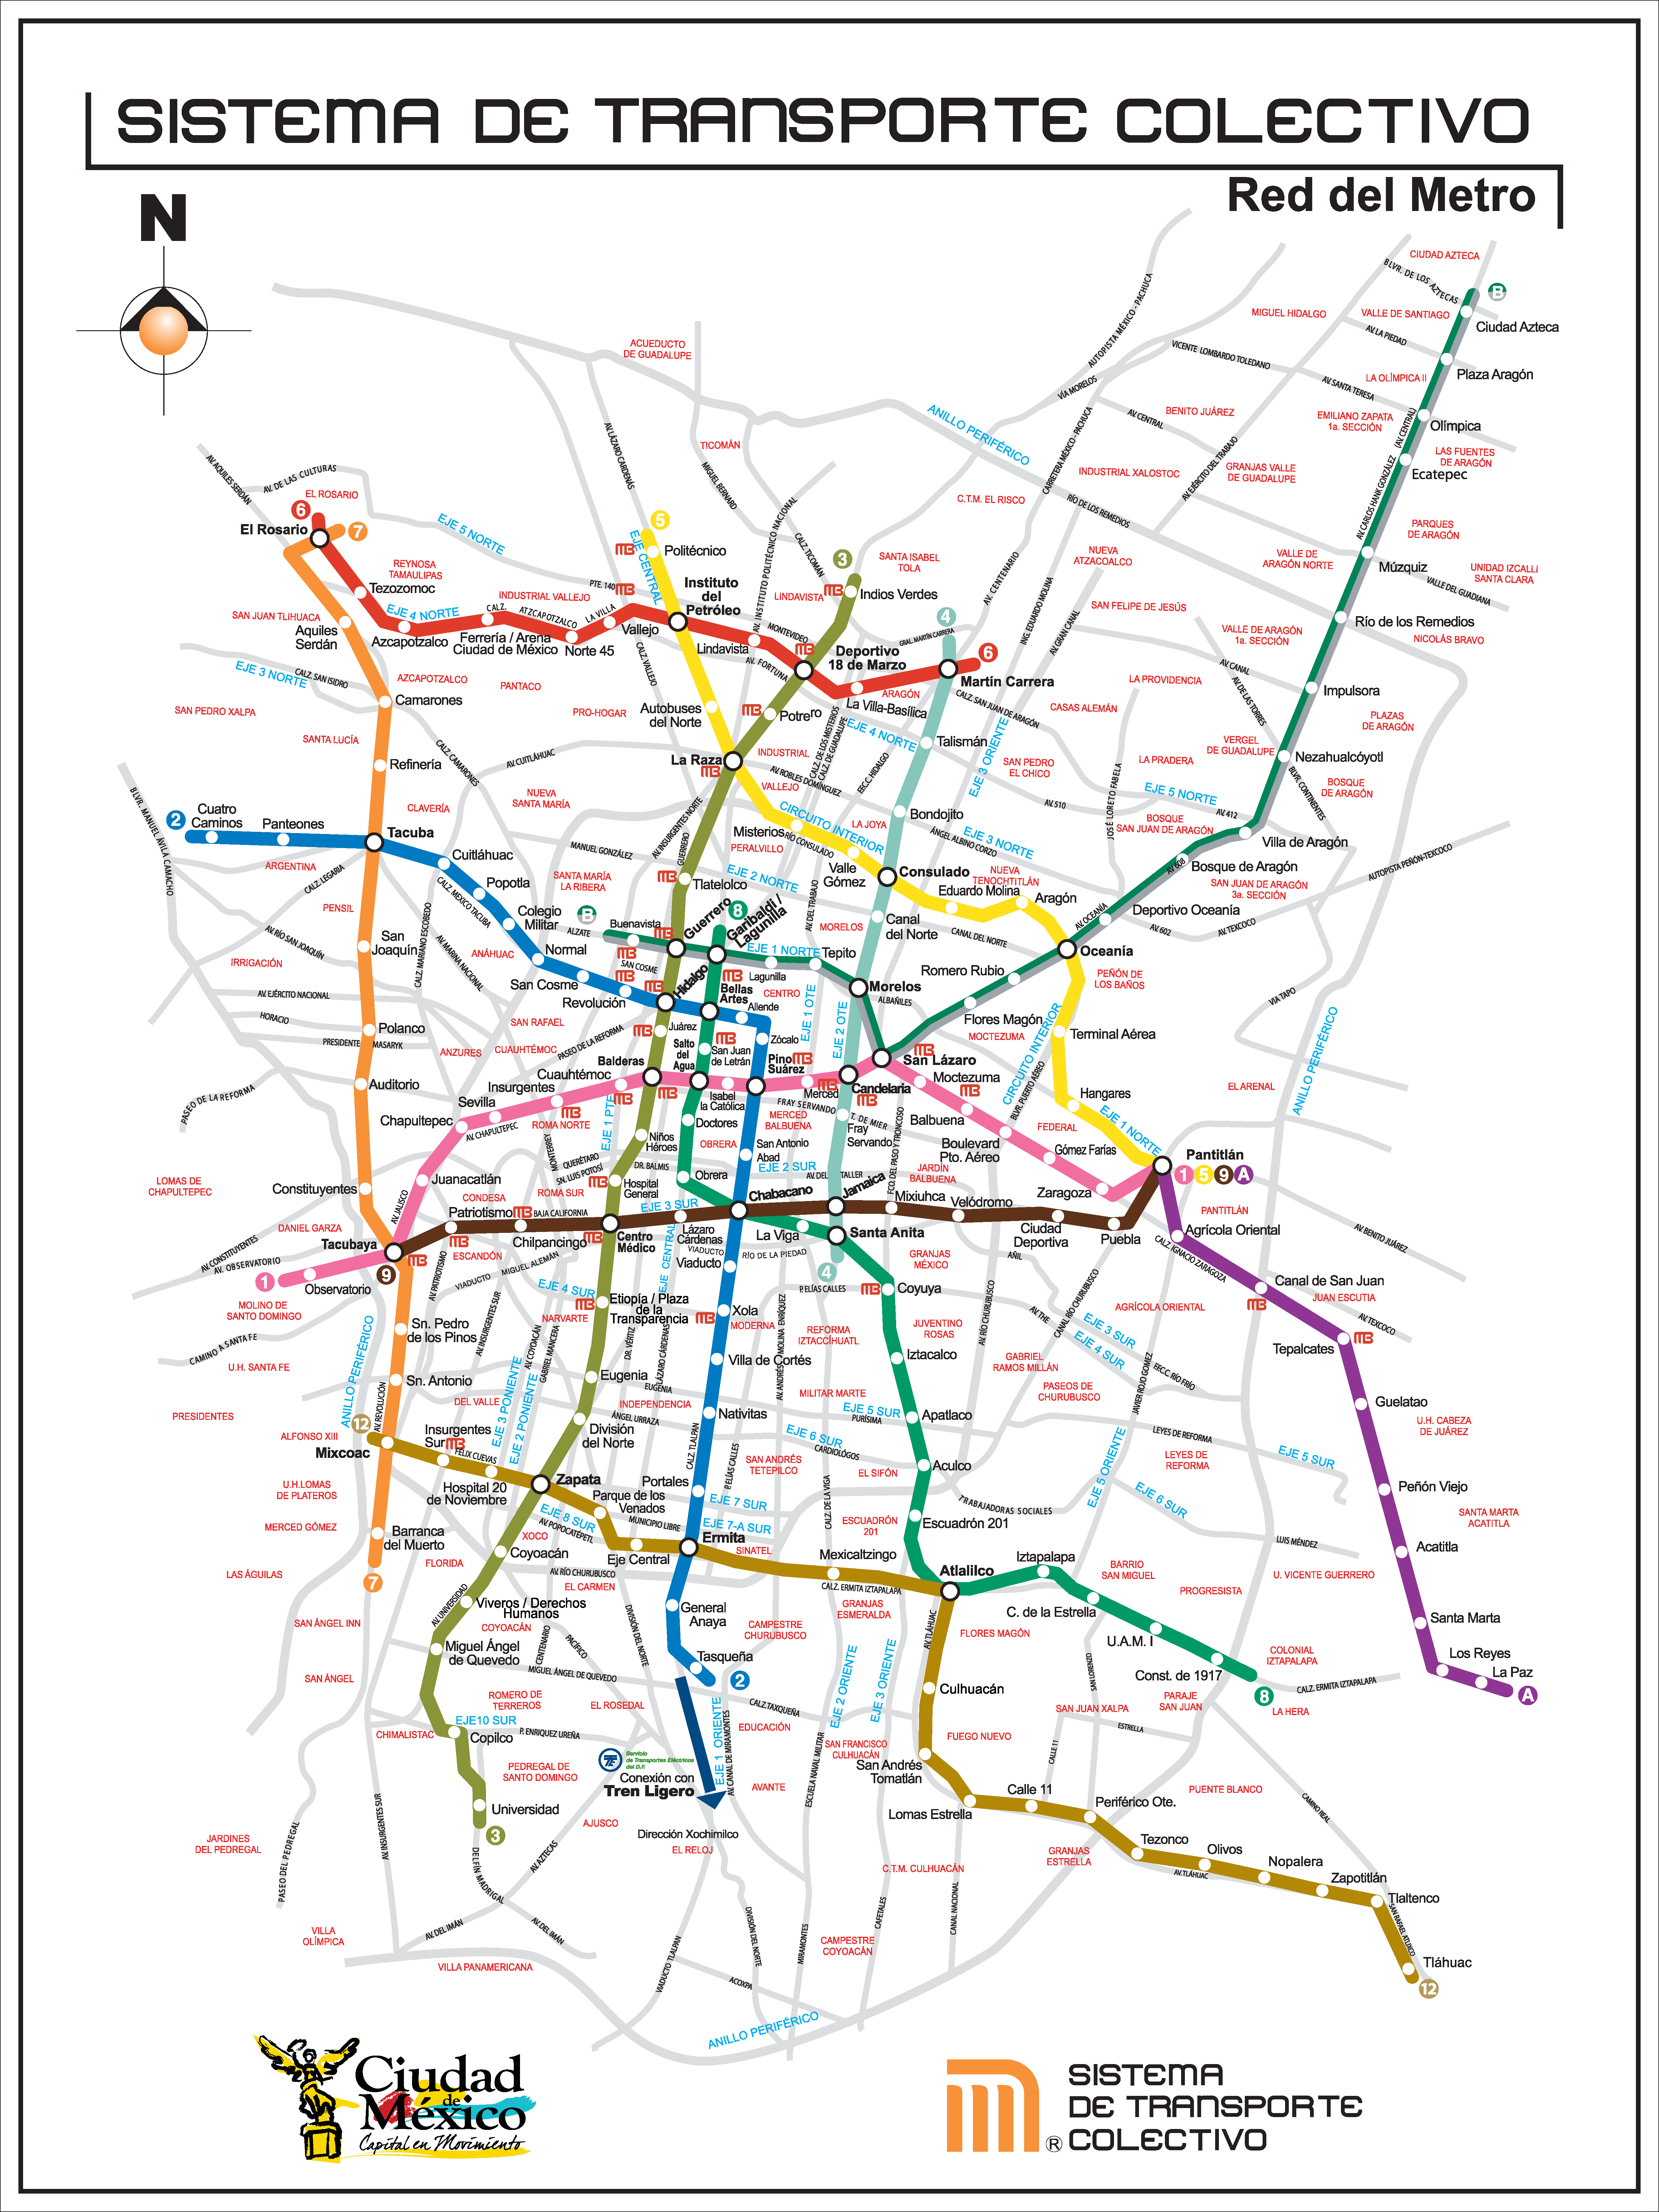
\includepdf[pages=-,scale=0.8,fitpaper=true]{pics/redinternet}
}

\section{Apéndice D. Expresiones para la actividad 13}

\begin{enumerate}
\item $a+b+c+d$
\item $a*(b-c)$
\item $a + a * (b − c) + (b − c) * d$
\item $i = i + 10$
\item $((x + y) − ((x + y) ∗ (x − y))) + ((x + y) ∗ (x − y))$
\item $a + b + (a + b)$
\item $a + b + a + b$
\item $a + a + ((a + a + a + (a + a + a + a))$
\end{enumerate}
\newpage

\section{Apéndice E. Mapa para la actividad 12}

{\centering
\includepdf[pages=-,offset=75 -75]{pics/archivo}
}

\newpage
\end{document}
